% Floe: technical report (IEEE conference format).
% Generated from main_template.tex by build_tex.py; numbers come from results/.
\documentclass[conference,a4paper]{IEEEtran}
\IEEEoverridecommandlockouts
\usepackage[T1]{fontenc}
\usepackage{graphicx}
\usepackage{booktabs}
\usepackage{array}
\usepackage{microtype}
\usepackage{amsmath}
\usepackage{xcolor}
\usepackage{listings}
\usepackage{url}
\usepackage[hidelinks]{hyperref}
\lstset{basicstyle=\ttfamily\scriptsize, columns=fullflexible, breaklines=true, frame=single,
        framerule=0.3pt, rulecolor=\color{black!40}, xleftmargin=2pt, xrightmargin=2pt, aboveskip=4pt, belowskip=4pt}
\newcommand{\code}[1]{\texttt{#1}}
\newcolumntype{L}[1]{>{\raggedright\arraybackslash}p{#1}}
\emergencystretch=1.5em

\begin{document}

\title{Floe: A Change-Data-Capture Lakehouse on Apache Iceberg, Spark and Trino}

\author{\IEEEauthorblockN{Aliyan Zulfiqar (Group Leader) \quad Sehrosh Riaz}
\IEEEauthorblockA{SE-315 Cloud Computing, Semester Project (Group 04)\\
Department of Computer Science, NBC\\
Instructor: Dr.\ Mohsin Raza Jafri \quad Lab Engineer: Engr.\ Muhammad Abid Hussain\\
Repository: \url{https://github.com/zorhehs/floe}}}

\maketitle

\begin{abstract}
Running analytics on an operational database competes with its transactions, and nightly batch exports deliver
stale data. We present Floe, a lakehouse that continuously replicates row-level changes from PostgreSQL into
Apache Iceberg tables and serves them to SQL analytics through Trino. Debezium reads the PostgreSQL write-ahead log
and publishes change events to Kafka; a Spark Structured Streaming job applies each micro-batch with an idempotent
\code{MERGE}, evolving table schemas automatically. Airflow orchestrates Spark maintenance jobs for partition
evolution, sorted compaction, snapshot expiry and GDPR-style erasure, and Prometheus and Grafana monitor freshness
and file health. On TPC-H scale factor~1 (1,650,030 rows) the full load became queryable at 4,844 rows/s
end to end, individual changes reached Trino with a median latency of 7.3\,s, and source and lakehouse matched
exactly by row-level checksums. Re-laying out the streamed tables removed all 105 merge-on-read delete
files, reduced stored objects by 89\% and made a suite of eight analytical queries 3.25$\times$ faster
overall.
\end{abstract}

\begin{IEEEkeywords}
lakehouse, change data capture, Apache Iceberg, Spark Structured Streaming, Debezium, Trino, compaction
\end{IEEEkeywords}

\section{Introduction and Motivation}
Organisations increasingly want analytics over the same data their applications are modifying: orders, balances
and inventory. Running heavy analytical SQL directly on the operational database competes with transaction
processing, while the traditional alternative of exporting full tables to a warehouse every night is costly, because
each run copies all data, and stale, because results can be a day old. A lakehouse combines low-cost open storage
with the transactional table semantics of a warehouse~\cite{armbrust2021}, and change data capture (CDC) feeds it
incrementally by reading only the changes recorded in the database log.

This project builds such a system, which we call \emph{Floe}, entirely from open-source components and measures its
behaviour. The objectives were to (i) stream inserts, updates and deletes from PostgreSQL into Apache Iceberg;
(ii) keep the copy correct and fresh, including across source schema changes; (iii) demonstrate schema evolution,
time travel and row-level deletion; (iv) counter the small-file problem caused by streaming writes with compaction
and partition optimisation orchestrated by Airflow, and quantify query performance and storage before and after; and
(v) make the system observable, reproducible and tested.

\section{Background}
\textbf{Change data capture.} PostgreSQL records every committed change in its write-ahead log (WAL). With
\code{wal\_level=logical}, a logical replication slot decodes the WAL into row changes~\cite{pglogical}. Debezium
consumes the slot through the built-in \code{pgoutput} plugin, first snapshots existing rows and then emits one event
per changed row containing the new row image, the operation, the commit time and the log sequence number
(LSN)~\cite{debezium}. Because the slot retains WAL until the consumer confirms it, changes are not lost while the
consumer is unavailable.

\textbf{Apache Iceberg} is an open table format in which a table is a tree of immutable files: Parquet data files,
delete files, manifests and a metadata file~\cite{iceberg}. A catalog stores an atomic pointer to the current
metadata file, and every commit produces a new snapshot. This provides ACID transactions with optimistic
concurrency, time travel, schema evolution by column identifier, and hidden partitioning whose specification can be
changed without rewriting existing data. Format version~2 adds row-level deletes: with \emph{merge-on-read}, an update
writes the new row and a small position-delete file instead of rewriting the affected data file.

\textbf{Engines.} Spark Structured Streaming processes Kafka in micro-batches with checkpointed
offsets~\cite{spark}; Trino is a distributed SQL engine that reads Iceberg tables directly from object
storage~\cite{trino}.

\section{System Architecture}
Fig.~\ref{fig:arch} shows the components and data flow. All services run as containers defined in a single
Docker Compose file. Table~\ref{tab:components} summarises the components and the reasons for choosing them.

\begin{figure*}[t]
\centering
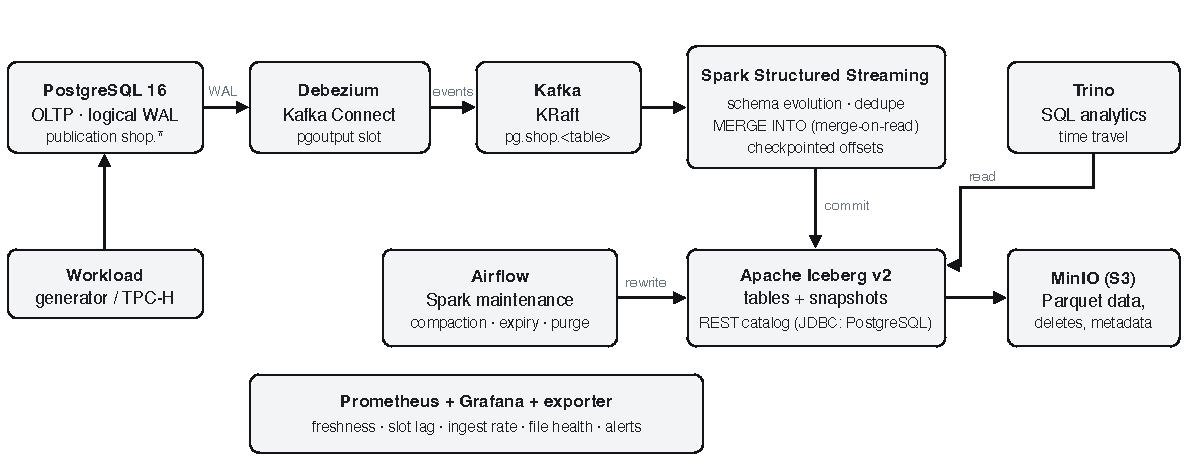
\includegraphics[width=0.86\textwidth]{figures/architecture.pdf}
\caption{Floe components and data flow.}
\label{fig:arch}
\end{figure*}

\begin{table}[t]
\caption{Components and design choices}
\label{tab:components}
\centering
\footnotesize
\begin{tabular}{@{}L{1.45cm}L{2.05cm}L{4.1cm}@{}}
\toprule
Layer & Component & Reason \\
\midrule
Source & PostgreSQL 16 & Logical decoding; publication covers future tables \\
CDC & Debezium 2.7 & Snapshot plus streaming; exact decimals with source precision \\
Transport & Kafka 3.9 (KRaft) & Durable, replayable log ordered per key \\
Processing & Spark 3.5 & \code{foreachBatch} gives full SQL (\code{MERGE}) per batch \\
Table format & Iceberg 1.9 (v2) & Engine-neutral; merge-on-read; partition evolution \\
Catalog & Iceberg REST & Standard API for Spark and Trino; state in PostgreSQL \\
Storage & MinIO & S3 API; replaceable by S3 or Azure Data Lake Storage \\
Query & Trino 476 & Interactive SQL, metadata tables, time travel \\
Orchestration & Airflow 2.10 & Scheduling, retries and history of maintenance jobs \\
Monitoring & Prometheus, Grafana & Pipeline-specific exporter and alert rules \\
\bottomrule
\end{tabular}
\end{table}

\section{Implementation}
\subsection{Change Capture}
An initialisation script creates separate database roles for the application, for Debezium (with the
\code{REPLICATION} attribute) and for the catalog, together with the TPC-H shaped schema \code{shop}. A publication
\code{FOR TABLES IN SCHEMA shop} includes tables created later. The connector is registered idempotently and uses
\code{decimal.handling.mode=string} with \code{column.propagate.source.type}, so that a \code{numeric(12,2)} column
arrives as an exact value together with its precision and scale. The setting \code{max\_slot\_wal\_keep\_size}
bounds the WAL that a stopped consumer can retain.

\subsection{Streaming Ingestion}
The Spark job subscribes to all topics of the schema and processes each micro-batch per table:
\begin{enumerate}
\item \emph{Schema discovery.} Each Debezium event carries its schema. The job collects the distinct schemas in the
batch by cutting the message text before the payload, which avoids parsing every event, and maps Debezium logical
types (dates, timestamps, decimals, binary) to Iceberg types.
\item \emph{Schema evolution.} Unknown tables are created as format-v2, merge-on-read tables. New source columns are
added with \code{ALTER TABLE ... ADD COLUMN}; promotions that Iceberg supports in place (integer to bigint, float to
double, wider decimal) are applied with \code{ALTER COLUMN ... TYPE}; other changes are cast and logged.
\item \emph{Deduplication.} Only the latest event per primary key, by Kafka offset, is kept.
\item \emph{Merge.} A single statement applies the batch:
\end{enumerate}
\begin{lstlisting}[language=SQL]
MERGE INTO lakehouse.shop.orders t USING batch s
  ON t.o_orderkey = s.o_orderkey
WHEN MATCHED AND s._cdc_op = 'd' THEN DELETE
WHEN MATCHED THEN UPDATE SET ...
WHEN NOT MATCHED AND s._cdc_op <> 'd' THEN INSERT ...
\end{lstlisting}
Because the statement is idempotent, replaying the last micro-batch after a failure yields the same table state,
which together with checkpointed offsets gives effectively-once results. Commits that conflict with a concurrent
maintenance job are retried with exponential backoff. Each row also stores the operation, the source commit time,
the LSN and the ingestion time, which are used to measure freshness and to audit changes.

\subsection{Maintenance and Orchestration}
A Spark job exposes the Iceberg maintenance procedures as composable steps, and three Airflow DAGs schedule them:
hourly housekeeping, a manual layout optimisation, and a GDPR purge. The layout optimisation partitions
\code{orders} by \code{months(o\_orderdate)}, sorts it by order date and customer, sorts \code{customer} by nation
and key, and then runs \code{rewrite\_data\_files} with the sort strategy, \code{rewrite\_position\_delete\_files},
\code{rewrite\_manifests}, \code{expire\_snapshots} and \code{remove\_orphan\_files}. Partition evolution changes only
metadata, so the streaming job continues without restarting. Orphan removal receives an S3 listing through
\code{file\_list\_view} and only deletes files older than 24\,h, which protects files of in-flight commits.

\subsection{Monitoring, Testing and Reproducibility}
A Prometheus exporter writes a heartbeat row into PostgreSQL every 15\,s and reports the age of the newest heartbeat
visible through Trino, which is the end-to-end freshness. It also reports replication-slot lag, connector state,
ingest rate, merge duration and the number of data and delete files per table (Fig.~\ref{fig:grafana}). Alert rules
cover stale data, a stopped connector, WAL growth, small-file accumulation and a stalled stream. Correctness is
checked by comparing row counts and an order-independent \code{checksum()} over all columns between the PostgreSQL
and Iceberg catalogs in Trino. The repository contains unit tests, a full-stack integration test, a GitHub Actions
workflow and scripts for setup, demonstration and clean-up.

\begin{figure}[t]
\centering
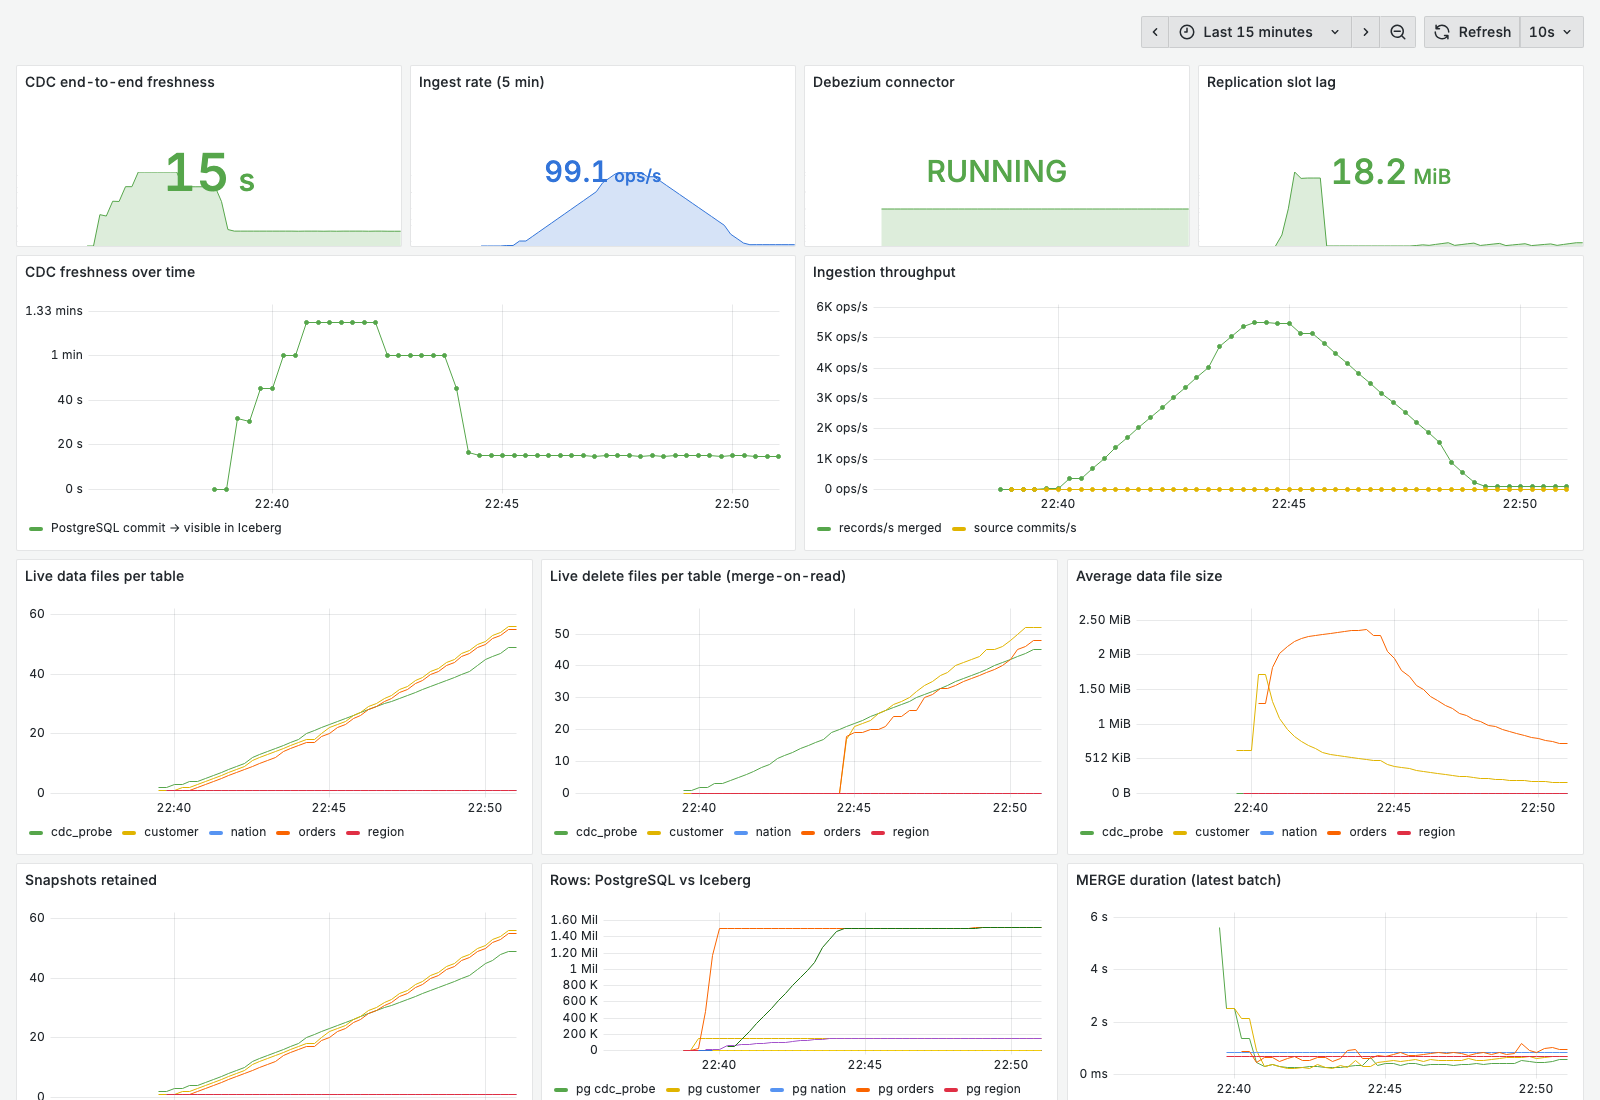
\includegraphics[width=\columnwidth]{figures/grafana_dashboard.png}
\caption{Grafana dashboard during the final run: the initial-load backlog drains, then freshness stays steady
under the live workload while data and delete files accumulate.}
\label{fig:grafana}
\end{figure}

\section{Evaluation}
\subsection{Setup}
All services ran on one laptop (Apple silicon, 8 cores) with Docker limited to 8\,GB of memory and Spark in local
mode, so the results describe a single node. The data set is TPC-H scale factor~1 (150\,000 customers and 1\,500\,000
orders) generated by Trino's \code{tpch} connector~\cite{tpch}, followed by a synthetic OLTP workload of 100
operations per second for five minutes (45\% new orders, 20\% order updates, 10\% order deletes, 15\% balance
updates, 5\% new and 5\% deleted customers). Spark used a 10\,s trigger and at most 100\,000 records per batch.
Query times are medians of 5 runs after one warm-up run.

\subsection{Ingestion Throughput}
Loading 1,650,030 rows into PostgreSQL took 27\,s, and all rows were queryable in Iceberg with matching
checksums 341\,s after the load started, i.e.\ 4,844 rows/s end to end. Over 62 micro-batches
(1,688,434 change events) the job processed 3,575 events/s while busy, with a peak of 7,752 events/s
and a median batch time of 3.7\,s (95th percentile 20.5\,s). The \code{MERGE} into \code{orders} took
0.9\,s at the median (1.9\,s at the 95th percentile) even for batches of about 90\,000 rows; most of the
batch time is spent decoding the self-describing JSON events on a single executor (Fig.~\ref{fig:ingest}).

\begin{figure}[t]
\centering
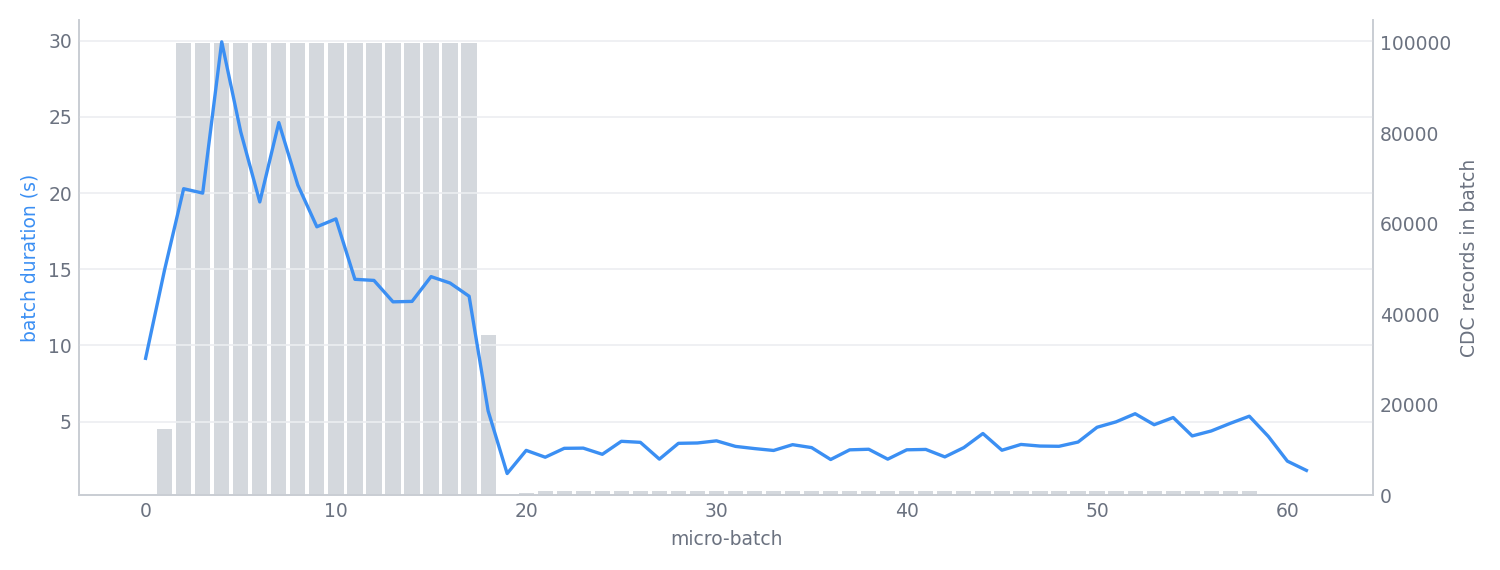
\includegraphics[width=\columnwidth]{figures/ingestion.png}
\caption{Change events (bars) and processing time (line) per micro-batch: initial load, then live workload.}
\label{fig:ingest}
\end{figure}

\subsection{End-to-End Freshness}
During the workload, probe rows were inserted into PostgreSQL every 2\,s and polled through Trino. All 40 probes
became visible (0 timed out); the time from commit to visibility had a median of 7.3\,s, a 95th
percentile of 11.7\,s and a maximum of 12.7\,s (Fig.~\ref{fig:fresh}). Freshness is bounded below by the
trigger interval plus the merge and commit time; a shorter trigger reduces latency at the cost of more and smaller
files.

\begin{figure}[t]
\centering
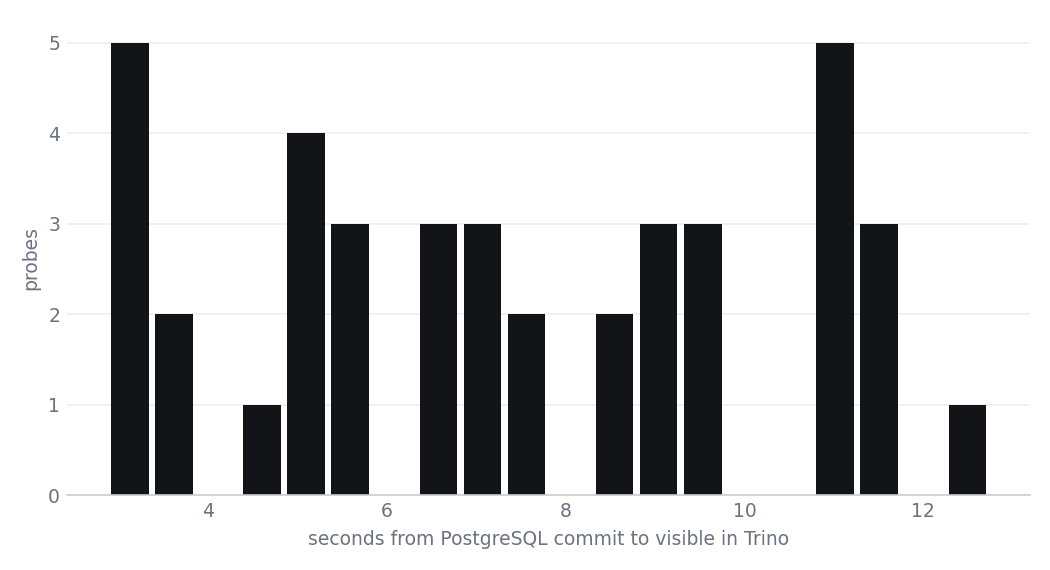
\includegraphics[width=0.92\columnwidth]{figures/freshness.png}
\caption{Distribution of end-to-end freshness (PostgreSQL commit to visible in Trino).}
\label{fig:fresh}
\end{figure}

\subsection{Layout Optimisation: Files, Storage and Queries}
After the load and workload, \code{orders} consisted of 57 data files averaging 717\,KB plus
49 position-delete files that every query must merge at read time. The optimisation DAG rewrote it into
80 sorted files (average 581\,KB) in monthly partitions and expired the superseded snapshots
(Table~\ref{tab:files}, Fig.~\ref{fig:files}). The number of objects in storage fell by 89\% (from
2,151 to 246), while total bytes changed by only -0.4\% (58.5\,MB to 58.3\,MB): five minutes
of workload produce small delete files, so the gain is in object count, which drives listing and planning cost on
object storage, rather than in bytes.

\begin{table}[t]
\caption{Live files before $\rightarrow$ after optimisation}
\label{tab:files}
\centering
\footnotesize
\begin{tabular}{@{}lllll@{}}
\toprule
Table & Data files & Delete files & Avg.\ file (KB) & Snapshots \\
\midrule
orders & 57 $\rightarrow$ 80 & 49 $\rightarrow$ 0 & 717 $\rightarrow$ 581 & 57 $\rightarrow$ 1 \\
customer & 58 $\rightarrow$ 1 & 56 $\rightarrow$ 0 & 157 $\rightarrow$ 8,630 & 58 $\rightarrow$ 1 \\
\bottomrule
\end{tabular}
\end{table}

\begin{figure*}[t]
\centering
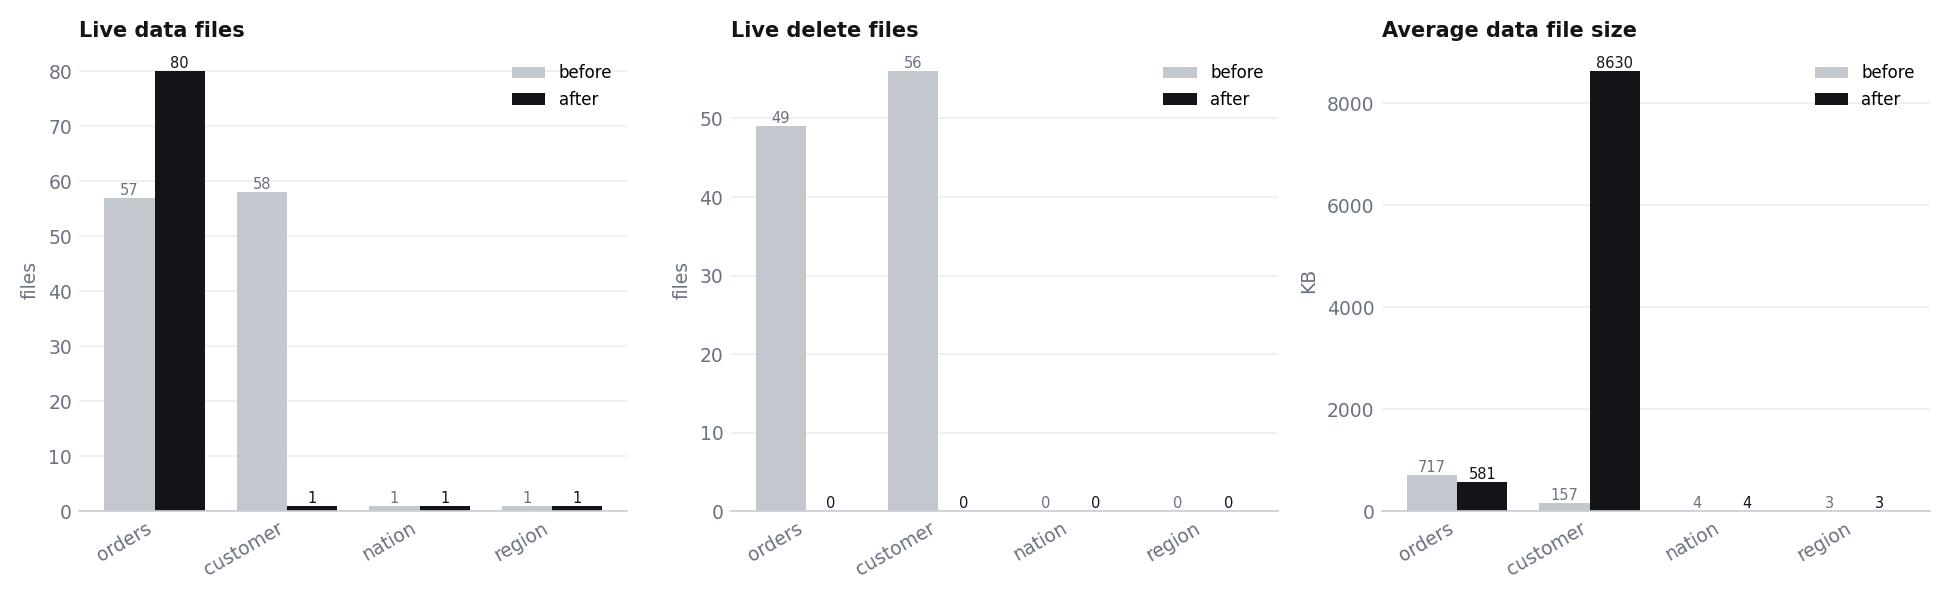
\includegraphics[width=0.9\textwidth]{figures/small_files.png}
\caption{Live data files, delete files and average data-file size per table before (grey) and after (black)
optimisation.}
\label{fig:files}
\end{figure*}

Table~\ref{tab:queries} compares the query suite. Overall the suite ran 3.25$\times$ faster, with the largest
gain for the point lookup query (8.8$\times$). Date-filtered queries benefit from partition pruning; the
single-month query read 19,488 rows instead of 1,513,192. Every query benefits from reading fewer files
without delete files to merge. Queries that did not improve: full aggregate (0.95$\times$). A whole-table scan gains nothing from pruning
and now opens more, smaller monthly files.

\begin{table}[t]
\caption{Trino query latency (median, ms) and rows read (millions)}
\label{tab:queries}
\centering
\footnotesize
\setlength{\tabcolsep}{3.2pt}
\begin{tabular}{@{}llrrrrr@{}}
\toprule
\# & Query & Before & After & Speed-up & Read bef. & Read aft. \\
\midrule
Q01 & point lookup & 971 & 110 & 8.81$\times$ & 1.23 & 1.51 \\
Q02 & single month & 340 & 46 & 7.38$\times$ & 1.51 & 0.02 \\
Q03 & quarterly revenue & 1,287 & 174 & 7.39$\times$ & 1.51 & 0.69 \\
Q04 & revenue by nation & 8,089 & 1,381 & 5.86$\times$ & 1.81 & 0.53 \\
Q05 & top customers & 8,934 & 3,646 & 2.45$\times$ & 1.81 & 1.81 \\
Q06 & full aggregate & 950 & 1,004 & 0.95$\times$ & 1.51 & 1.51 \\
Q07 & segment priority & 750 & 178 & 4.22$\times$ & 1.69 & 0.23 \\
Q08 & customer history & 240 & 91 & 2.64$\times$ & 1.49 & 1.51 \\
\midrule
 & \textbf{total} & \textbf{21,561} & \textbf{6,630} & \textbf{3.25$\times$} & & \\
\bottomrule
\end{tabular}
\end{table}

\textbf{Partition granularity.} An ablation on an already compacted table compared one compacted file with the same
data in monthly partitions (80 files of about 570\,KB). Partitioning changed the one-month query
latency by -18\%, but slowed the full-table queries by +21\% and +35\%. At scale factor~1 a month
holds only about 20\,000 orders; monthly partitions pay off as volume grows, while at small scale a coarser transform
or a sort order alone is preferable. Partition evolution makes this a metadata-only decision.

\subsection{Compaction Overhead}
The complete optimisation DAG took 170\,s of wall time while the streaming job kept running
(Table~\ref{tab:tasks}). Most of the time is Spark start-up and the per-table orphan scan; the sorted rewrite of
\code{orders} itself took well under a minute.

\begin{table}[t]
\caption{Optimisation DAG task durations}
\label{tab:tasks}
\centering
\footnotesize
\begin{tabular}{@{}lr@{}}
\toprule
Airflow task & Duration (s) \\
\midrule
apply\_layout\_and\_compact & 43.9 \\
rewrite\_deletes\_and\_manifests & 22.8 \\
expire\_snapshots & 23.1 \\
remove\_orphan\_files & 67.7 \\
\bottomrule
\end{tabular}
\end{table}

\subsection{Fault Tolerance and Correctness}
During an earlier freshness measurement the Docker virtual machine ran out of memory and the operating system killed
the Spark driver. The container restarted, resumed from the checkpointed offsets and re-applied the interrupted
batch; because the merge is idempotent no change was lost or duplicated. Median freshness in that run remained
10.8\,s, but probes caught in the restart took up to 78.6\,s. Memory limits were reduced afterwards. Row
counts and checksums of every table matched between PostgreSQL and Iceberg before and after optimisation
(Table~\ref{tab:cons}), and the same check passed after the initial load, after the workload, after replaying the
Kafka topics into an empty lake, and in the integration test.

\begin{table}[t]
\caption{PostgreSQL versus Iceberg (row-level checksum)}
\label{tab:cons}
\centering
\footnotesize
\begin{tabular}{@{}lrl@{}}
\toprule
Table & Rows & Before / after optimisation \\
\midrule
customer & 149,932 & match / match \\
nation & 25 & match / match \\
orders & 1,513,192 & match / match \\
region & 5 & match / match \\
\bottomrule
\end{tabular}
\end{table}

\subsection{Functional Demonstrations}
Adding a column and widening an integer column to bigint in PostgreSQL reached Iceberg within about 10\,s as
metadata-only changes. Time-travel queries by snapshot identifier and by timestamp returned the earlier values of an
updated order. A customer deleted in PostgreSQL disappeared from current queries within about 10\,s but remained
readable through time travel until the purge DAG rewrote the affected files and expired the history.

\section{Technical Challenges and Lessons Learned}
Several problems appeared only under realistic load. Concurrent commits made the REST catalog's SQLite store return
\code{SQLITE\_BUSY}; moving catalog state to PostgreSQL solved it. Spark \code{MERGE} failed on Iceberg tables with
identifier fields, so the primary key is stored as a table property instead. \code{remove\_orphan\_files} requires a
Hadoop file system for S3, which the stack does not include, so the file listing is supplied through
\code{file\_list\_view}. Default memory sizing of Trino, Kafka Connect and the maintenance job caused failures during
the 1.5-million-row load and rewrite; explicit heap limits, a byte-bounded Debezium queue and spill-to-disk fixed them.
Finally, the sum of container memory exceeded the 8\,GB virtual machine, which led to the driver restart described
above. The main lesson is that the operational aspects of CDC ingestion (concurrent writers, metadata growth, small
files and observability) matter as much as the data path, and that a repeatable correctness check makes each of them
easier to resolve.

\section{Conclusion and Future Work}
Floe makes changes from PostgreSQL queryable in Iceberg within seconds, keeps an exact copy of the source, evolves
schemas without intervention, supports time travel and verifiable erasure, and uses scheduled optimisation to turn
streaming-induced small files into a layout that made the query suite 3.25$\times$ faster while reducing stored
objects by 89\%. The evaluation is limited to a single node, freshness is bounded by the micro-batch trigger,
and dropped source columns remain in Iceberg. Future work includes a comparison with Apache Hudi on the same
workload, column-level lineage with Apache Atlas, Avro with a schema registry to reduce serialisation cost, a
Kubernetes deployment on Azure with Data Lake Storage and Event Hubs, and Apache Flink for lower-latency ingestion.

\begin{thebibliography}{9}
\bibitem{armbrust2021} M.~Armbrust, A.~Ghodsi, R.~Xin, and M.~Zaharia, ``Lakehouse: A new generation of open platforms
that unify data warehousing and advanced analytics,'' in \emph{Proc. CIDR}, 2021.
\bibitem{iceberg} Apache Software Foundation, ``Apache Iceberg table specification and Spark procedures,''
\url{https://iceberg.apache.org/docs/latest/}.
\bibitem{debezium} Debezium, ``Debezium connector for PostgreSQL,'' version 2.7, \url{https://debezium.io/documentation/}.
\bibitem{pglogical} PostgreSQL Global Development Group, ``Logical replication,'' PostgreSQL 16 documentation.
\bibitem{spark} Apache Software Foundation, ``Structured Streaming programming guide,'' Spark 3.5,
\url{https://spark.apache.org/docs/3.5.6/}.
\bibitem{trino} Trino Software Foundation, ``Iceberg connector,'' \url{https://trino.io/docs/current/connector/iceberg.html}.
\bibitem{kafka} Apache Software Foundation, ``Apache Kafka documentation,'' version 3.9.
\bibitem{airflow} Apache Software Foundation, ``Apache Airflow documentation,'' version 2.10.
\bibitem{tpch} Transaction Processing Performance Council, ``TPC Benchmark H standard specification.''
\end{thebibliography}

\appendices
\section{Reproducing the Results}
\begin{lstlisting}[language=bash]
git clone https://github.com/zorhehs/floe && cd floe
./scripts/setup.sh            # checks, .env, jars, images
./scripts/run_demo.sh --full  # stack, TPC-H sf1, workload,
                              # validation, demos, benchmark
# or step by step
make up && make load && make bench && make validate
python3 docs/report/latex/build_tex.py   # rebuild this paper
\end{lstlisting}

\section{Key Configuration}
\begin{lstlisting}
# Debezium connector (config/debezium/postgres-cdc.json, excerpt)
plugin.name=pgoutput  publication.name=dbz_publication
slot.name=debezium_shop  topic.prefix=pg  snapshot.mode=initial
decimal.handling.mode=string  column.propagate.source.type=shop\..*
max.queue.size.in.bytes=134217728  heartbeat.interval.ms=10000

# Iceberg table properties set by the streaming job
format-version=2  write.{delete,update,merge}.mode=merge-on-read
write.parquet.compression-codec=zstd

# Layout optimisation (src/topologies/spark/maintenance.py)
ALTER TABLE lakehouse.shop.orders ADD PARTITION FIELD months(o_orderdate);
ALTER TABLE lakehouse.shop.orders WRITE ORDERED BY o_orderdate, o_custkey;
CALL lakehouse.system.rewrite_data_files(table => 'shop.orders',
  strategy => 'sort', options => map('rewrite-all','true',
  'target-file-size-bytes','134217728','partial-progress.enabled','true'));
\end{lstlisting}

\end{document}
